
\svnid{$Id: $}
\svnid{$URL: $}

\section{FOR REVIEW:Storage curve of channels with rectangular profiles (storage)}
\newrefsegment

%---------------------------------------------------------------------------------
\section*{Quality Assurance}
\begin{tabular}{@{}p{27mm}@{}p{0mm}p{\textwidth-52mm-48pt}p{15mm}p{10mm}}
\textbf{Date} & \textbf{:} &   November 1 2019\\ 
\textbf{Author} & \textbf{:} & Eskedar Gebremedhin  & \textbf{Initials:} & E.T \\
\textbf{Review} & \textbf{:} &   & \textbf{Initials:} & \ldots 
\end{tabular}

%---------------------------------------------------------------------------------
\section*{Version information}
{{
\begin{tabular}{@{}p{27mm}@{}p{0mm}p{\textwidth-27mm-24pt}}
\textbf{Executable}   & \textbf{:} & Deltares, D-Flow FM 1.2.76.65238M, November 1 2019, 15:14:31  \\
\textbf{Location input}     & \textbf{:} & \url{https://repos.deltares.nl/repos/DSCTestbench/trunk/cases/e02_dflowfm/f105_cross-sections/c11_rectangular-profile-storage} \\
\textbf{Revision input} & \textbf{:} & - \\
\textbf{Location output}     & \textbf{:} & \url{https://repos.deltares.nl/repos/DSCTestbench/trunk/references/win64/e02_dflowfm/f105_cross-sections/c11_rectangular-profile-storage} \\
\textbf{Revision output} & \textbf{:} & -
\end{tabular}
}}

%---------------------------------------------------------------------------------
\section*{Purpose}
The purpose of this validation test is to verify that the proper functioning of the rectangular cross-sectional profiles with a focus on the storage curve.

%---------------------------------------------------------------------------------
\section*{Linked claims}
\begin{enumerate}
\item \dflowfm can take into account the shape of several cross sectional profiles (circle, rectangle, ZW, XYZ and YZ).
\end{enumerate}

%---------------------------------------------------------------------------------
\section*{Approach}

The model includes a horizontal uniform channel, a sloping channel, and a horizontal widening channel with rectangular profiles.
A constant discharge is imposed at the eastern (low) boundary to slowly fill up the channels like bathtubs.
The water levels as function of time are compared to the analytical solution at a number of locations, namely near inflow boundary.
The analytical solution for the water level is derived from a calculation of the relationship of the storage (taking into account varying profile shape and slope) in the systems and the cumulative inflow.

%---------------------------------------------------------------------------------
\section*{Conclusion} 
Proper functioning of rectangular profiles where it relates to storage is confirmed. 
The modelled storage curves extracted from varied locations in the sub-models are identical to the analytical solution after a spin-up period during which numerical drying-flooding thresholds play a role.
%---------------------------------------------------------------------------------
\section*{Model description}

The test comprises of three separate sub-models (see \autoref{fig:e02_f105_c11_layout}) with the following characteristics.

\begin{itemize}
	\item All models are 2000 m in length with an equidistant grid spacing of 50 m. 
	\item All models have a constant hydraulic roughness of Ch\'ezy = 45 m\textsuperscript{1/2}/s.       
	\item The eastern boundary condition for T1 and T3  models is a {constant} discharge of 0.04 m$^3$/s and for T2 0.02  m$^3$/s.
	\item The western boundary is closed for all models such that the inflowing water slowly fills up in the system. 
	\item T1 is a model with a constant rectangular profile (4 m width and 3 m height) with a flat bed at $z$ = 0 m AD.
	\item T2 is a model with a constant rectangular profile (4 m width and 3 m height) with a sloped bed (3 m AD at the western boundary and 0 m AD at the eastern boundary). Note that the inflow boundary is located at the lower eastern boundary.
	\item T3 is a model with a widening rectangular profile (at the eastern boundary with 4 m width and 3 m height and at the western boundary with 6 m width and 3 m height) with a flat bed at $z$ = 0 m AD.
\end{itemize}

\textbf{Note:} \dflowfm simulations add an additional half grid spacing at the ends of the system to implement the flow boundary conditions at the center of the link. The cross-sectional profiles of these segments are uniform and are extended from the profiles at the end of the section. The analytical solution does account for this.

\begin{figure}[H]
    \centering
	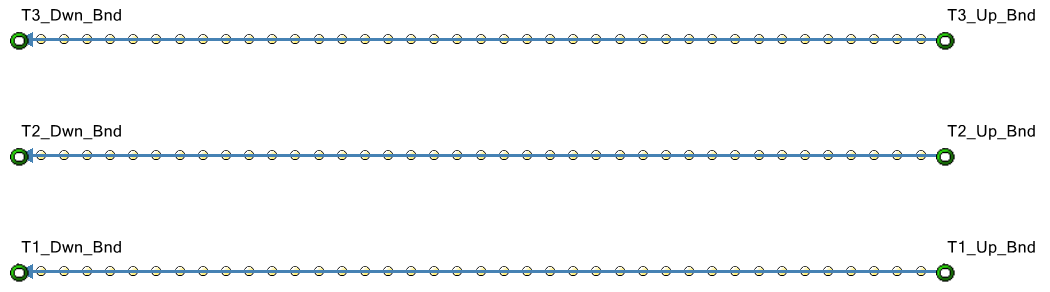
\includegraphics[width=.95\linewidth]{figures/e02_f105_c11_layout.PNG}
	\caption{Lay-out of the test model, equidistant grid spacing at connection nodes}
	\label{fig:e02_f105_c11_layout}
\end{figure}

Note that \dflowfm simulations add an additional half grid spacing at the ends of the system to implement the flow boundary conditions at the center of the link. 
The cross-sectional profiles of these segments are uniform and are extended from the profiles at the end of the section. 
The analytical solution does account for this.

%---------------------------------------------------------------------------------
\section*{Results}
The storage curve, water level as function of storage (=integrated inflow) volume, is extracted at the eastern (inflow) boundary (chainage=0). 
These results are compared with the analytical solution in \autoref{fig:e02_f105_c11_T1results} to \autoref{fig:e02_f105_c11_T3results}

\begin{figure}[H]
    \centering
    \includegraphics*[width=0.95\textwidth]{figures/e02_f105_c11_submodel_T1_results.jpg}
    \caption{Analytical and modelled storage curves at sub-model {T1}}
    \label{fig:e02_f105_c11_T1results}
\end{figure} 

\begin{figure}[H]
    \centering
    \includegraphics*[width=0.95\textwidth]{figures/e02_f105_c11_submodel_T2_results.jpg}
    \caption{Analytical and modelled storage curves at sub-model {T2}}
    \label{fig:e02_f105_c11_T2results}
\end{figure} 

\begin{figure}[H]
    \centering
    \includegraphics*[width=0.95\textwidth]{figures/e02_f105_c11_submodel_T3_results.jpg}
    \caption{Analytical and modelled storage curves at sub-model {T3}}
    \label{fig:e02_f105_c11_T3results}
\end{figure} 

%---------------------------------------------------------------------------------
\section*{Analysis of results}

The system is filled slowly through a small discharge from the eastern boundary ensuring steady and uniformity in the system. 
Water levels at all chainage locations in a sub-model should therefore be equal at any time (after a short spin-up period during which the drying-flooding threshold causes the water to be distributed over a smaller part of the model than the analytical solution indicates). 
A comparison of the storage curves extracted from different locations in all sub-models is in line with this expectation.

The analytical and modelled storage curves are identical for all sub-models apart from the spin-up period at the start of the simulation. 

%---------------------------------------------------------------------------------
\printrefsegment
